\documentclass[a4paper, 12pt]{article}

% Paquete de idioma
\usepackage[spanish, es-nodecimaldot, mexico]{babel} % mexico es para que aparezca en laa leyenda de tablas y no cuadros en las tablas.

\usepackage[utf8]{inputenc}

%Fecha
\usepackage[useregional]{datetime2}

% Configuración de página
\usepackage{geometry}
\geometry{left = 15mm, right = 15mm, top=35mm, bottom=20mm, headheight=30mm, showframe} % showframe muestra los marcos de las páginas

% Paquete para justificar el texto
\usepackage{ragged2e}

% Referencias
\usepackage{hyperref} % Para hacer hipervínculos
\hypersetup{colorlinks=true, linkcolor=colorAzul1, citecolor=cyan, urlcolor=colorAzul1, linktocpage, hyperfootnotes=true} % Para que aprezca de color rojo por defecto los hipervínculos al poner linkcolor=blue cambia a color azul las referencias

% Paquetes de fuentes
\usepackage{courierten}
\renewcommand*\familydefault{\ttdefault} %% Only if the base font of the document is to be typewriter style
\usepackage[T1]{fontenc}

% Paquetes de colores
\usepackage[table]{xcolor} % Table es para utilizar los colores en tablas también.
\definecolor{colorRojo1}{rgb}{1.0, 0.03, 0.0}
\definecolor{colorAzul1}{rgb}{0.0, 0.75, 1.0}
\definecolor{colorGris1}{rgb}{0.75, 0.75, 0.75}
\definecolor{colorGris2}{rgb}{0.66, 0.66, 0.66}
\definecolor{colorGris3}{RGB}{50, 50, 50}

% Encabezados
\usepackage{lastpage}
\usepackage{fancyhdr}
\pagestyle{fancy}

\color{colorGris1}\renewcommand{\headrulewidth}{0.5mm}
\let\oldheadrule\headrule % Pone como comando antiguo
\renewcommand{\headrule}{\color{colorAzul1}\oldheadrule} % Redefine el comando anterior en sí está sobreescribiendo el comando anterior del encabezado
\renewcommand{\footrulewidth}{0.2mm}
\let\oldfootrule\footrule % Pone como comando antiguo
\renewcommand{\footrule}{\color{colorAzul1}\oldfootrule} % Redefine el comando anterior en sí está sobreescribiendo el comando anterior del pie de página

% Pie de página
\lfoot{\textcolor{colorGris2} {\small \titulo}}
\cfoot{}
\rfoot{\textcolor{colorGris2}{\small Página. \thepage\ / \pageref*{LastPage}}} % El asterisco en pageref es para que no se genere el hipervínculo y tenga otro color}

% Encabezado
\lhead{
\includegraphics[width=0.15\textwidth]{logox}}
\chead{\autor}
\rhead{Domingo \DTMsetstyle{ddmmyyyy}\fechainicio}
\usepackage{setspace} % Permite separar entre línea de texto con mucha soltura.
\usepackage{titlesec} % Para editar las secciones
\titleformat{\section}{\color{colorAzul1}\normalfont\Large\bfseries}{\thesection}{1em}{}
\titleformat{\subsection}{\color{colorAzul1}\normalfont\large\bfseries}{\thesubsection}{1em}{}

% Paquetes de figuras
\usepackage{graphicx} % Carga las figuras
\graphicspath{{./Figuras}} % Indica la dirección de las figuras
\usepackage{float} % Permite poner la posición H
\usepackage{subcaption} % Permite poner subfiguras
\usepackage{wrapfig} % Para envolver el texto alrededor de la figura
\usepackage{overpic} % Para poner texto sobre las figuras
\usepackage{caption} % Para las mini páginas poner etiquetas
\usepackage{tikz} % Para cargar el fondo de la portada
\usepackage[font={color = colorAzul1}]{caption} % Para el color de los captions

% Paquete de tablas
\usepackage{booktabs} % Para darle varios tipos de líneas en las tablas
\usepackage{colortbl} % Para darle color a las tablas


% Paquete para ecuaciones matemáticas
\usepackage{mathtools}

% Bibliografía
\usepackage[backend=biber, style=apa, sortcites, url=true]{biblatex} % Para las bibliografías y no salga el error de compilacion bcf
\addbibresource{Bibliografia/biblio_1.bib} % Poner la extensión es importante y recordar que los nombres de archivos o carpetas no tengan símbolos como tildes, espacios, etc. en estilo se puede poner alfabético, apa, etc.
\urlstyle{sf}

\begin{document}
	% Comandos personalizados
	\newcommand{\fechainicio}{\DTMdate{2024-02-25}}
	\newcommand{\fechafinal}{\DTMdate{2024-03-09}}
	\newcommand{\titulo}{NOTAS SOBRE LATEX}
	\newcommand{\autor}{Luis ZG}
	\renewcommand{\contentsname}{Contenido} % Para poner contenido en vez de índice
	\renewcommand{\tablename}{\bfseries Tabla} % Para poner la etiqueta o leyenda de tabla 
	\renewcommand{\figurename}{\bfseries Figura} % Para poner la etiqueta o leyenda de figura
	\renewcommand{\thefootnote}{\textcolor{colorAzul1}{\arabic{footnote}}}
	
	\color{colorGris3}
	\begin{titlepage}
		\thispagestyle{empty} % Desaparece encabezado y pie de página
		\begin{tikzpicture}[remember picture, overlay] % El texto se supepone encima de la figura.
			\node[inner sep=0pt] at (current page.center)
			{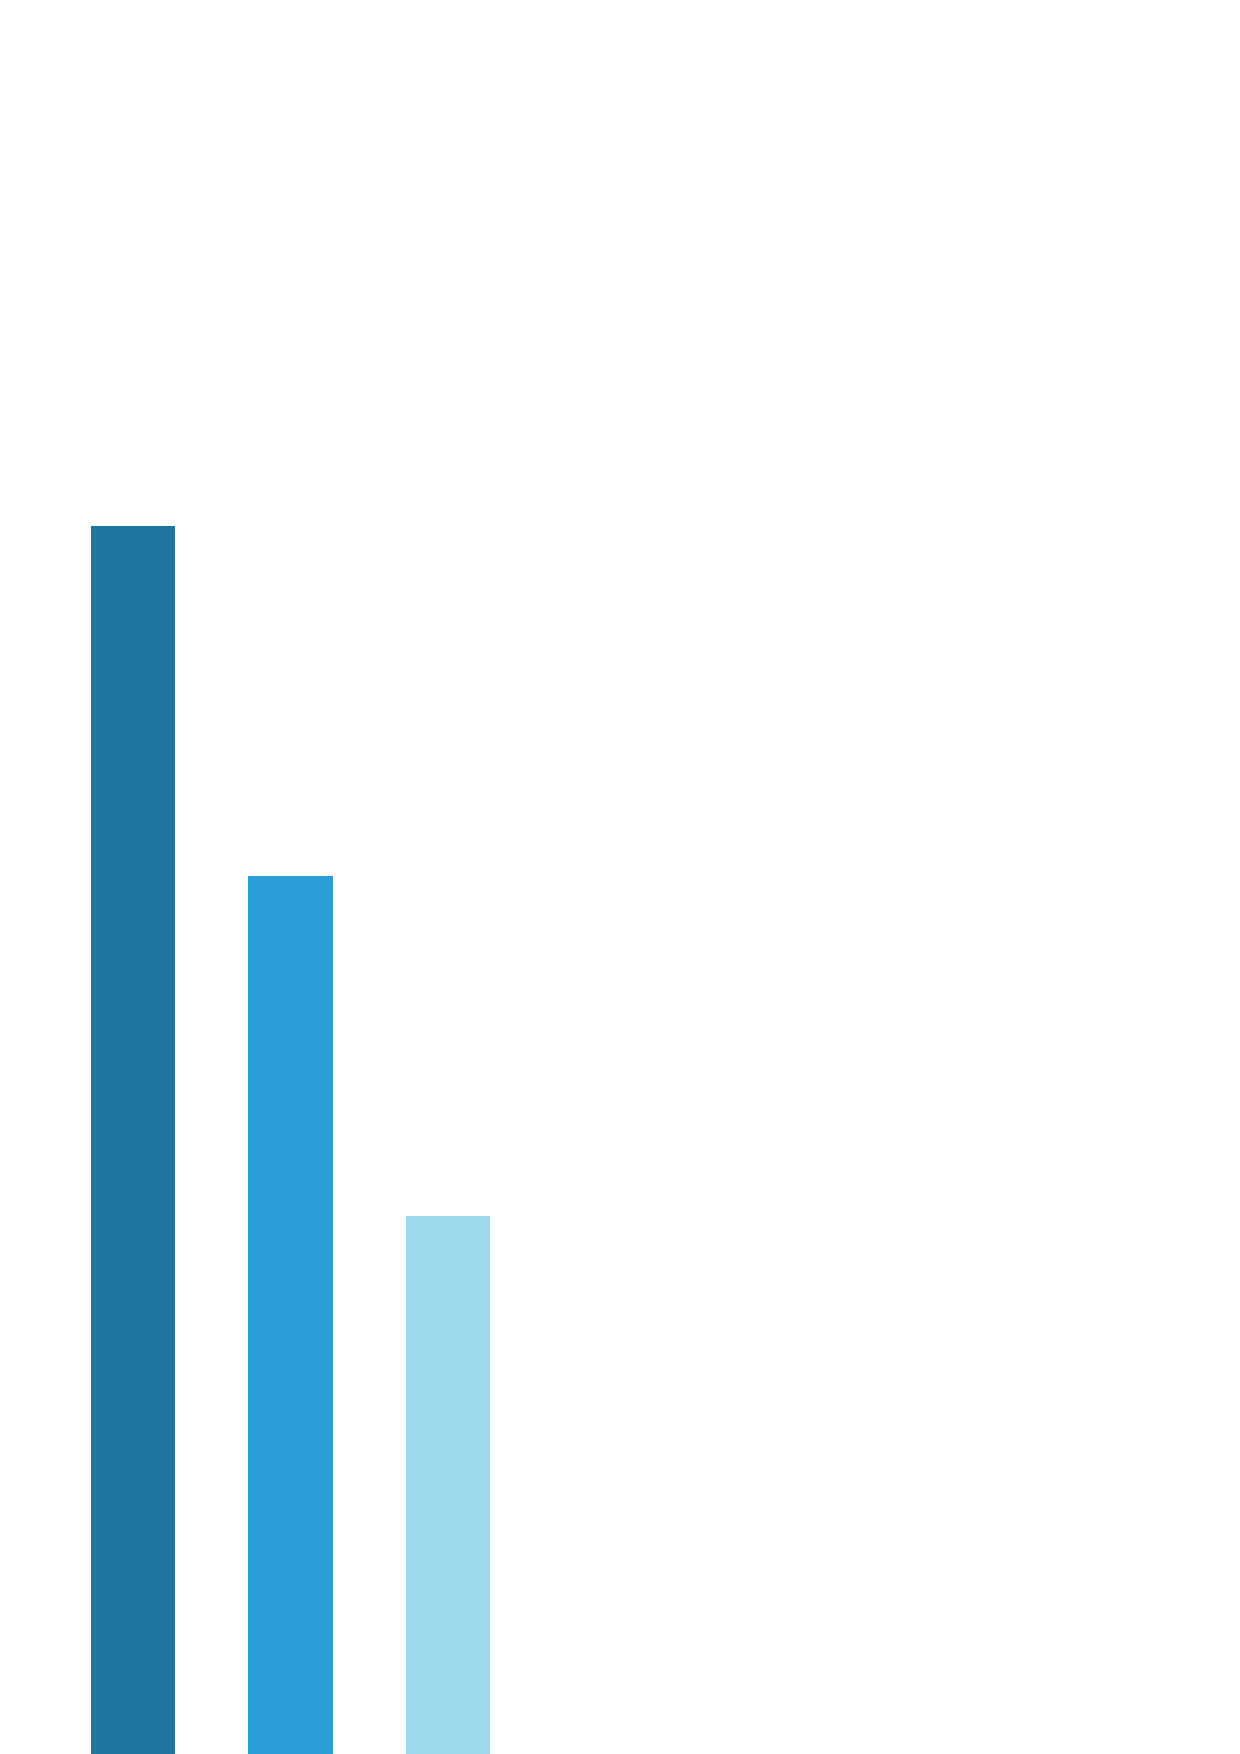
\includegraphics[width=21cm]{cover.pdf}};
		\end{tikzpicture}
		
		
		\hfill
		\begin{minipage}{8cm}
			\vspace{5cm}
			\begin{flushright}
				\begin{spacing}{3}
					{\fontsize{40}{50} \selectfont \color{colorRojo1} \textbf{\titulo}}
				\end{spacing}
			\end{flushright}
		\end{minipage}
		\vfill
		\hfill
		\begin{minipage}{10cm}
			\begin{flushright} \color{colorGris1}
				\begin{spacing}{2}
					
					\color{colorAzul1} \textbf{Manual de ayuda}
					
					\color{colorAzul1} \underline {Por: \autor.}
					
					Inicio: Domingo \fechainicio
					
					Fin: Sábado \fechafinal
				\end{spacing}
			\end{flushright}
		\end{minipage}
		
	\end{titlepage}
	
	\newpage
	\color{colorAzul1} \tableofcontents
	\newpage
	
	\begin{flushleft} \color{colorGris2}
		
		\section{Comandos rápidos}
		
		Ctrl + flechaDerecha: Cambia de opción en el editor TeXstudio.\newline
		
		Ctrl + clic: Lleva a la palabra que pertenece entre editor y el PDF.\newline
		
		Ctrl + t: Comenta todo el código seleccionado
		
		\textbackslash indent: Inserta sangría.\newline
		
		\textbackslash noindent: Elimina sangría.\newline
		
		\textbackslash textbackslash: Inserta el carácter \textbackslash.\newline
		
		\textbackslash \%: Inserta el símbolo de porcentaje.\newline
		
		\textbackslash \$: Inserta el símbolo del dólar.\newline
		
		\textbackslash \#: Inserta el símbolo del numeral.\newline
		
		\textbackslash \&: Inserta el símbolo del and.\newline
		
		\textbackslash \_: Inserta el símbolo sub guion.\newline
		
		\section{Configuración del documento}
		
		Comando: \textbackslash documentclass[a4paper, 11pt]\{article\}\newline
			
		Acción: Configura el documento  a formato de hoja A4, con tamaño de texto 11pt en tipo de documento artículo.\newline
			
		\section{Entorno del documento}
			
		Comando: \textbackslash begin\{document\}\newline
		Aquí van los párrafos del documento.\newline
		\textbackslash end\{document\}\newline
			
		Acción: Todos los entorno empieza con Begin y terminan con end y el nombre del entorno entre corchetes.\newline
		
		\section{Paquete de colores}
		
		Comando: \textbackslash usepackage\{xcolor\}\newline
		\textbackslash definecolor\{rojo1\}\{rgb\}\{1.0, 0.03, 0.0\}\newline
		\textbackslash definecolor\{azul1\}\{rgb\}\{0.0, 0.75, 1.0\}\newline
		\textbackslash definecolor\{gris1\}\{rgb\}\{0.75, 0.75, 0.75\}\newline
		\textbackslash definecolor\{gris2\}\{rgb\}\{0.66, 0.66, 0.66\}\newline
			
		Acción: Sirve para configurar los colores que se utilizará en el documento.\newline
		
		\section{Paquete de fuentes}
			
		Comando: \textbackslash renewcommand*\textbackslash ttdefault\{lcmtt\}\newline
		\textbackslash renewcommand*\textbackslash familydefault\{\textbackslash ttdefault\}\newline
		\textbackslash usepackage[OT1]\{fontenc\}\newline
			
		Acción: Sirve para personalizar las fuentes del documento.\newline
		
		\section{Paquete de idioma}
			
		Comando: \textbackslash usepackage[spanish, es-nodecimaldot]\{babel\}\newline
		\textbackslash usepackage[utf8]\{inputenc\}\newline
			
		Acción: Sirve para indicarle a TeXstudio que estamos trabajando en el idioma español con la configuración utf8, el paquete de idiomas se llama babel, el parámetro es-nodecimaldot es para que el separador de decimales sea el punto y no  la coma.\newline
		
		\section{Secciones}
		
		Comando: \textbackslash section\{nombre de la sección\}\newline
		
		Acción: Sirve para generar secciones numeradas, si se desea que no  se vea el número, el comando  sería \textbackslash section*\{Secciones\} tener cuidado no ponerle asterisco a la primera sección.\newline
		
		\section{Índice}
		
		Comando: \textbackslash tableofcontents\newline
		
		Acción: Sirve para generar el índice, para actualizar el índice se debe compilar 2 veces.\newline
		
		\section{Salto de página}
		
		\subsection{Comando 1:} \textbackslash newpage\newline
		\subsection{Comando 2:} \textbackslash clearpage\newline
		
		Acción: Sirve para hacer saltos de páginas y para figuras y elementos flotantes se recomienda clearpage.\newline
		
		\section{Listas no numeradas}
		
		Comando: \textbackslash begin\{itemize\}\newline
		\textbackslash item hola1\newline
		\textbackslash item hola2\newline
		\textbackslash end\{itemize\}\newline
		
		Acción: Sirve para generar listas no numeradas, si se desea una sub lista se hace lo mismo de la lista y si se desea cambiar el símbolo del inicio de las líneas de las listas en los ítem sepone paréntesis así: \textbackslash item[-].\newline
		
		\section{Listas numeradas}
		
		Comando: \textbackslash begin\{enumerate\}\newline
		\textbackslash item hola1\newline
		\textbackslash item hola2\newline
		\textbackslash end\{enumerate\}\newline
		
		Acción: Sirve para generar listas enumeradas.\newline
		
		\section{Listas con descripción}
		
		Comando: \textbackslash begin\{description\}\newline
		\textbackslash item[Descripción 1] Esta es la descripción 1.\newline
		\textbackslash item[Descripción 2] Esta es la descripción 2.\newline
		\textbackslash end\{description\}\newline
		
		Acción: Sirve para generar listas con descripciones y estas generan sangrias si el texto es muy extenso.\newline
		
		\section{Figuras}
		
		Comando: \textbackslash usepackage\{graphicx\}\newline
		\textbackslash graphicspath\{\{./Figuras\}\}\newline
		
		Acción: graphicx sirve para cargar las figuras y graphicspath sirve para indicar la dirección de las figuras.\newline
		
		\begin{figure}[h]
			\centering
			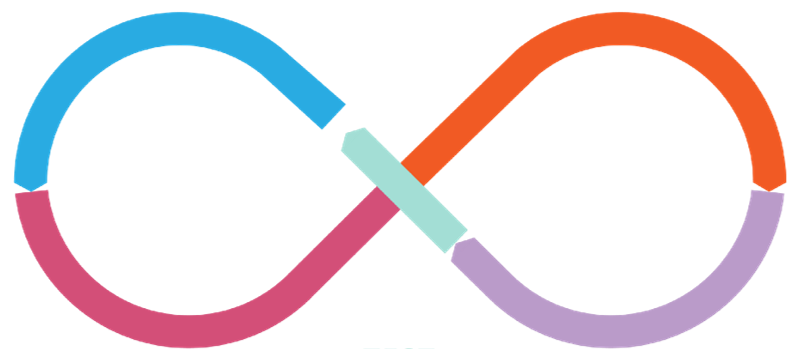
\includegraphics[width=0.25\textwidth]{flujo}
			\caption{Representación del infinito}
			\label{fig:flujo1}
		\end{figure}
		
		\begin{minipage}{0.99\textwidth}
			
			sfsdafa sagdgdf ggfdg gdfg gd gfdg gfgsgf ggsfg ggsdfg jhgjghjhk kjhgkhgkhg khgkhgkgh kjhkhkggkh khgkhgkh vxcvx cvxcv xcbcbvc bvcbv cbcvvnv nbmbn mnbmn bmn bmnb nbmnbmnb mn mnb mnbmbnmnb.
			
			\begin{wrapfigure}{l}{0.25\textwidth}
				\centering
				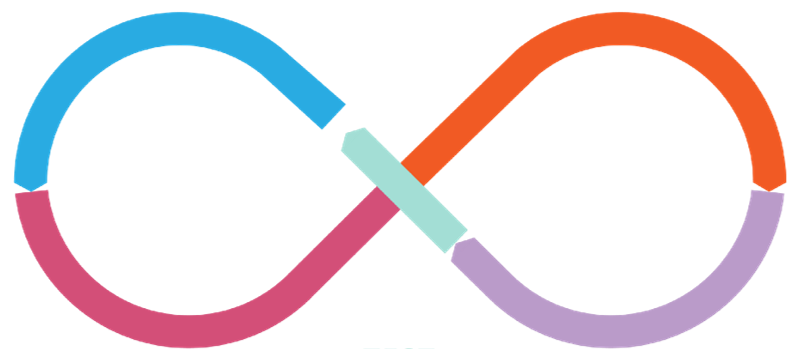
\includegraphics[width=0.9\linewidth]{flujo}
				\caption{Representación del infinito}
				\label{fig:flujo2}
			\end{wrapfigure}
			
			ggfdg gdfg gd gfdg gfgsgf ggsfg ggsdfg jhgjghjhk kjhgkhgkhg khgkhgkgh kjhkhkggkh khgkhgkh vxcvx cvxcv xcbcbvc bvcbv cbcvvnv nbmbn mnbmn bmn bmnb nbmnbmnb mn mnb mnbmbnmnb.
			
			sfsdafa sagdgdf ggfdg gdfg gd gfdg gfgsgf ggsfg ggsdfg jhgjghjhk kjhgkhgkhg khgkhgkgh kjhkhkggkh khgkhgkh vxcvx cvxcv xcbcbvc bvcbv cbcvvnv nbmbn mnbmn bmn bmnb nbmnbmnb mn mnb mnbmbnmnb.
			
			\begin{wrapfigure}{r}{0.25\textwidth}
				\centering
				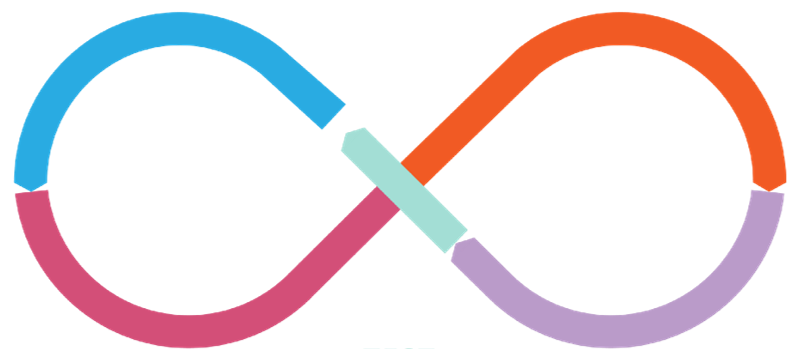
\includegraphics[width=0.9\linewidth]{flujo}
				\caption{Representación del infinito}
				\label{fig:flujo3}
			\end{wrapfigure}
			
			sfsdafa sagdgdf ggfdg gdfg gd gfdg gfgsgf ggsfg ggsdfg jhgjghjhk kjhgkhgkhg khgkhgkgh kjhkhkggkh khgkhgkh vxcvx cvxcv xcbcbvc bvcbv cbcvvnv nbmbn mnbmn bmn bmnb nbmnbmnb mn mnb mnbmbnmnb.
			
			dgdfgd gdffg sfdgfdgdfg gdfgdf
			
			ggfdg gdfg gd gfdg gfgsgf ggsfg ggsdfg jhgjghjhk kjhgkhgkhg khgkhgkgh kjhkhkggkh khgkhgkh vxcvx cvxcv xcbcbvc bvcbv cbcvvnv nbmbn mnbmn bmn bmnb nbmnbmnb mn mnb mnbmbnmnb.
			
			sfsdafa sagdgdf ggfdg gdfg gd gfdg gfgsgf ggsfg ggsdfg jhgjghjhk kjhgkhgkhg khgkhgkgh kjhkhkggkh khgkhgkh vxcvx cvxcv xcbcbvc bvcbv cbcvvnv nbmbn mnbmn bmn bmnb nbmnbmnb mn mnb mnbmbnmnb.
		\end{minipage}
		
		
		\section{Figuras que flotan}
		Ver en la imagen figura \autoref{fig:flujo4}.
		\begin{figure}[H]
			\centering
			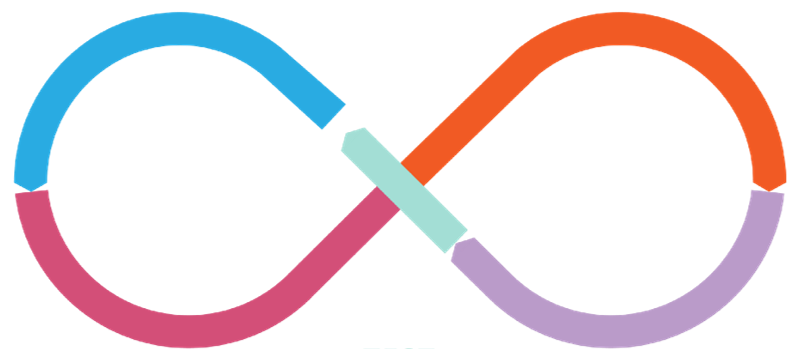
\includegraphics[width=0.6\linewidth]{flujo}
			\caption{Imagen sobre el infinito}
			\label{fig:flujo4}
		\end{figure}
		ggfdg gdfg gd gfdg gfgsgf ggsfg ggsdfg jhgjghjhk kjhgkhgkhg khgkhgkgh kjhkhkggkh khgkhgkh vxcvx cvxcv xcbcbvc bvcbv cbcvvnv nbmbn mnbmn bmn bmnb nbmnbmnb mn mnb mnbmbnmnb.
		
		
		\section{Dos figuras}
		ggfdg gdfg gd gfdg gfgsgf ggsfg ggsdfg jhgjghjhk kjhgkhgkhg khgkhgkgh kjhkhkggkh khgkhgkh vxcvx cvxcv xcbcbvc bvcbv cbcvvnv nbmbn mnbmn bmn bmnb nbmnbmnb mn mnb mnbmbnmnb.
		ggfdg gdfg gd gfdg gfgsgf ggsfg ggsdfg jhgjghjhk kjhgkhgkhg khgkhgkgh kjhkhkggkh khgkhgkh vxcvx cvxcv xcbcbvc bvcbv cbcvvnv nbmbn mnbmn bmn bmnb nbmnbmnb mn mnb mnbmbnmnb.
		
		\begin{figure}[h]
			\centering
			
\includegraphics[width=0.2\linewidth]{grafica_torta}
			\caption{La torta}
			\label{fig:torta1}
		\end{figure}
		
		\begin{figure}[h]
			\centering
			
\includegraphics[width=0.2\linewidth]{grafica_barras}
			\caption{Las barras}
			\label{fig:barra1}
		\end{figure}
		
		\begin{figure}[h]
			\centering
			\begin{subfigure}{0.45\textwidth}
				\centering
				
\includegraphics[width=0.4\linewidth]{grafica_torta}
				\caption{Una torta}
				\label{subtorta1}
			\end{subfigure}\hfil % Distribulle uniformemente las figuras y con hfill el espacio de enmedio se agranda
			\begin{subfigure}{0.45\textwidth}
				\centering
				
\includegraphics[width=0.4\linewidth]{grafica_barras}
				\caption{Unas barras}
				\label{subbarra1}
			\end{subfigure}
			\caption{Este es el caso donde se pueden poner 2 o más subfiguras la torta \ref{subtorta1} y las barras \ref{subbarra1}.}
			\label{fig:Dos subfiguras}
		\end{figure}
		
		ggfdg gdfg gd gfdg gfgsgf ggsfg ggsdfg jhgjghjhk kjhgkhgkhg khgkhgkgh kjhkhkggkh khgkhgkh vxcvx cvxcv xcbcbvc bvcbv cbcvvnv nbmbn mnbmn bmn bmnb nbmnbmnb mn mnb mnbmbnmnb.
		ggfdg gdfg gd gfdg gfgsgf ggsfg ggsdfg jhgjghjhk kjhgkhgkhg khgkhgkgh kjhkhkggkh khgkhgkh vxcvx cvxcv xcbcbvc bvcbv cbcvvnv nbmbn mnbmn bmn bmnb nbmnbmnb mn mnb mnbmbnmnb.
	\end{flushleft}	
	
	
	\begin{minipage}{0.99\textwidth}
	
	\section{Texto al lado de una figura}
	ggfdg gdfg gd gfdg gfgsgf ggsfg ggsdfg jhgjghjhk kjhgkhgkhg khgkhgkgh kjhkhkggkh khgkhgkh vxcvx cvxcv xcbcbvc bvcbv cbcvvnv nbmbn mnbmn bmn bmnb nbmnbmnb mn mnb mnbmbnmnb.
	\begin{wrapfigure}[10]{l}{0.3\linewidth}
		\vspace{-5mm}
		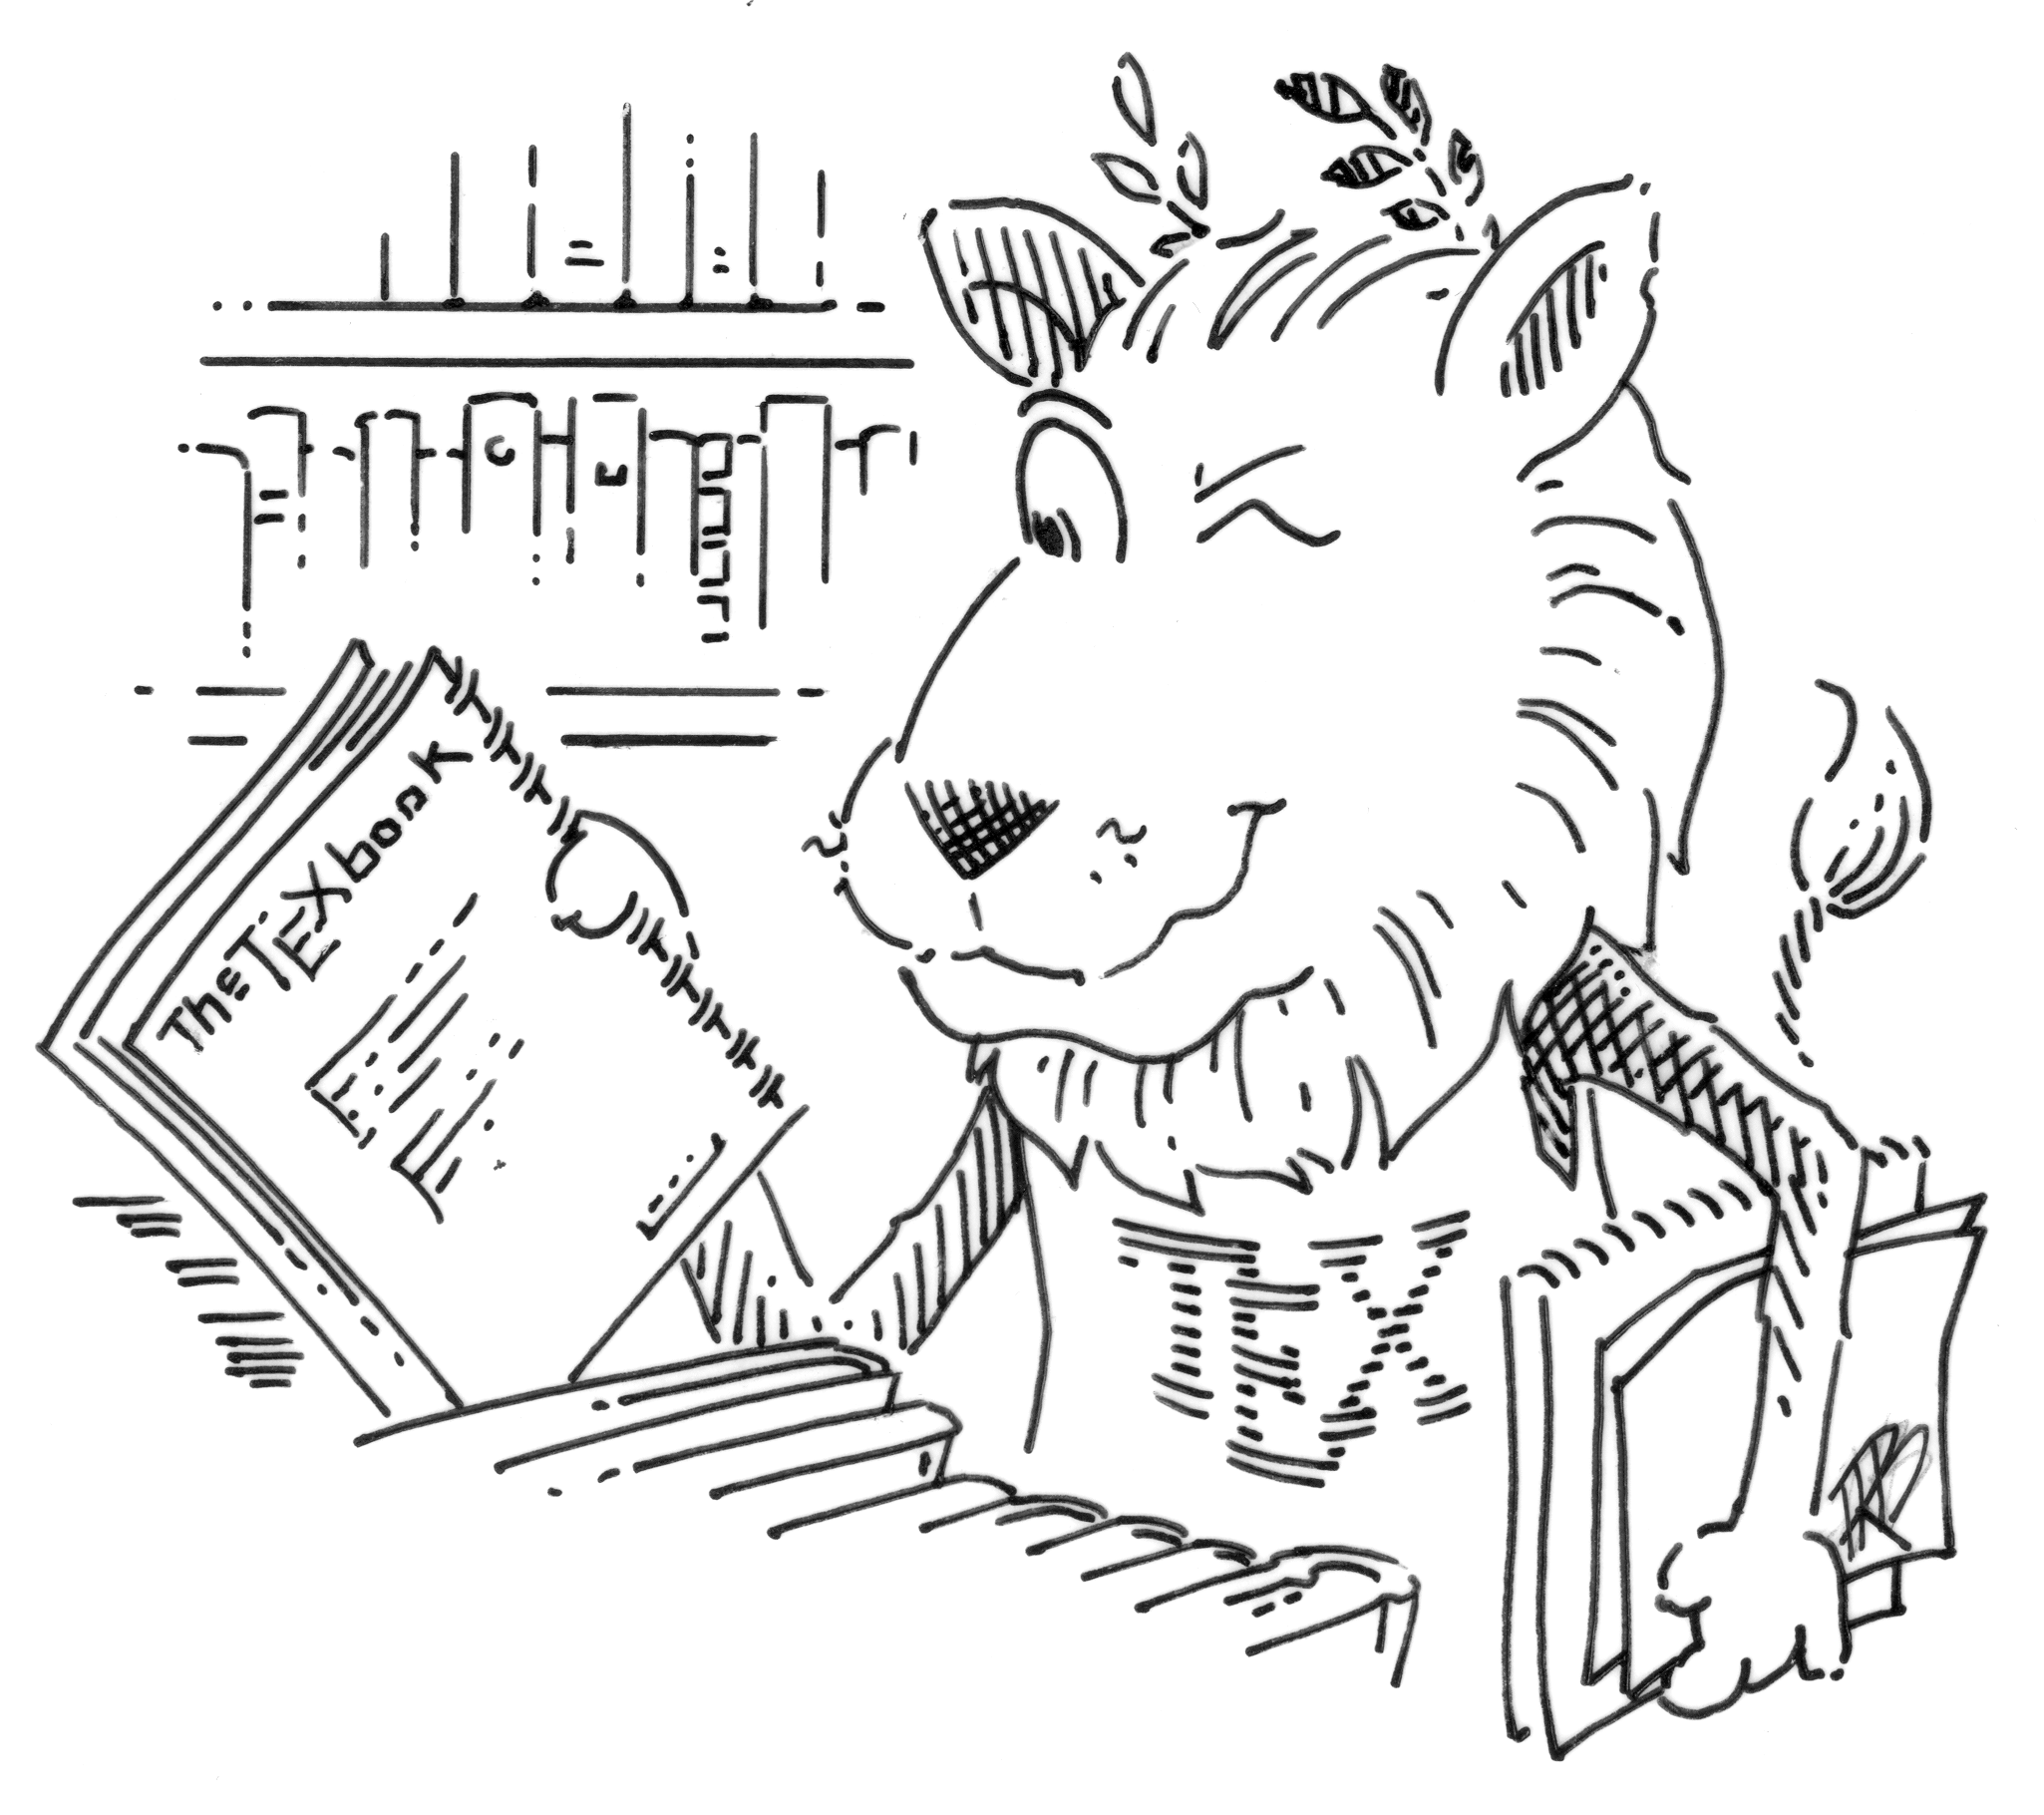
\includegraphics[width=0.8\linewidth]{tex_lion}
		\caption{El león Tex}
		\label{fig:leontex1}
	\end{wrapfigure}
	ggfdg gdfg gd gfdg gfgsgf ggsfg ggsdfg jhgjghjhk kjhgkhgkhg khgkhgkgh kjhkhkggkh khgkhgkh vxcvx cvxcv xcbcbvc bvcbv cbcvvnv nbmbn mnbmn bmn bmnb nbmnbmnb mn mnb mnbmbnmnb.
	
	
	ggfdg gdfg gd gfdg gfgsgf ggsfg ggsdfg jhgjghjhk kjhgkhgkhg khgkhgkgh kjhkhkggkh khgkhgkh vxcvx cvxcv xcbcbvc bvcbv cbcvvnv nbmbn mnbmn bmn bmnb nbmnbmnb mn mnb mnbmbnmnb.
	ggfdg gdfg gd gfdg gfgsgf ggsfg ggsdfg jhgjghjhk kjhgkhgkhg khgkhgkgh kjhkhkggkh khgkhgkh vxcvx cvxcv xcbcbvc bvcbv cbcvvnv nbmbn mnbmn bmn bmnb nbmnbmnb mn mnb mnbmbnmnb.
	ggfdg gdfg gd gfdg gfgsgf ggsfg ggsdfg jhgjghjhk kjhgkhgkhg khgkhgkgh kjhkhkggkh khgkhgkh vxcvx cvxcv xcbcbvc bvcbv cbcvvnv nbmbn mnbmn bmn bmnb nbmnbmnb mn mnb mnbmbnmnb.
	\begin{wrapfigure}[8]{r}{0.3\linewidth}
		\vspace{-5mm}
		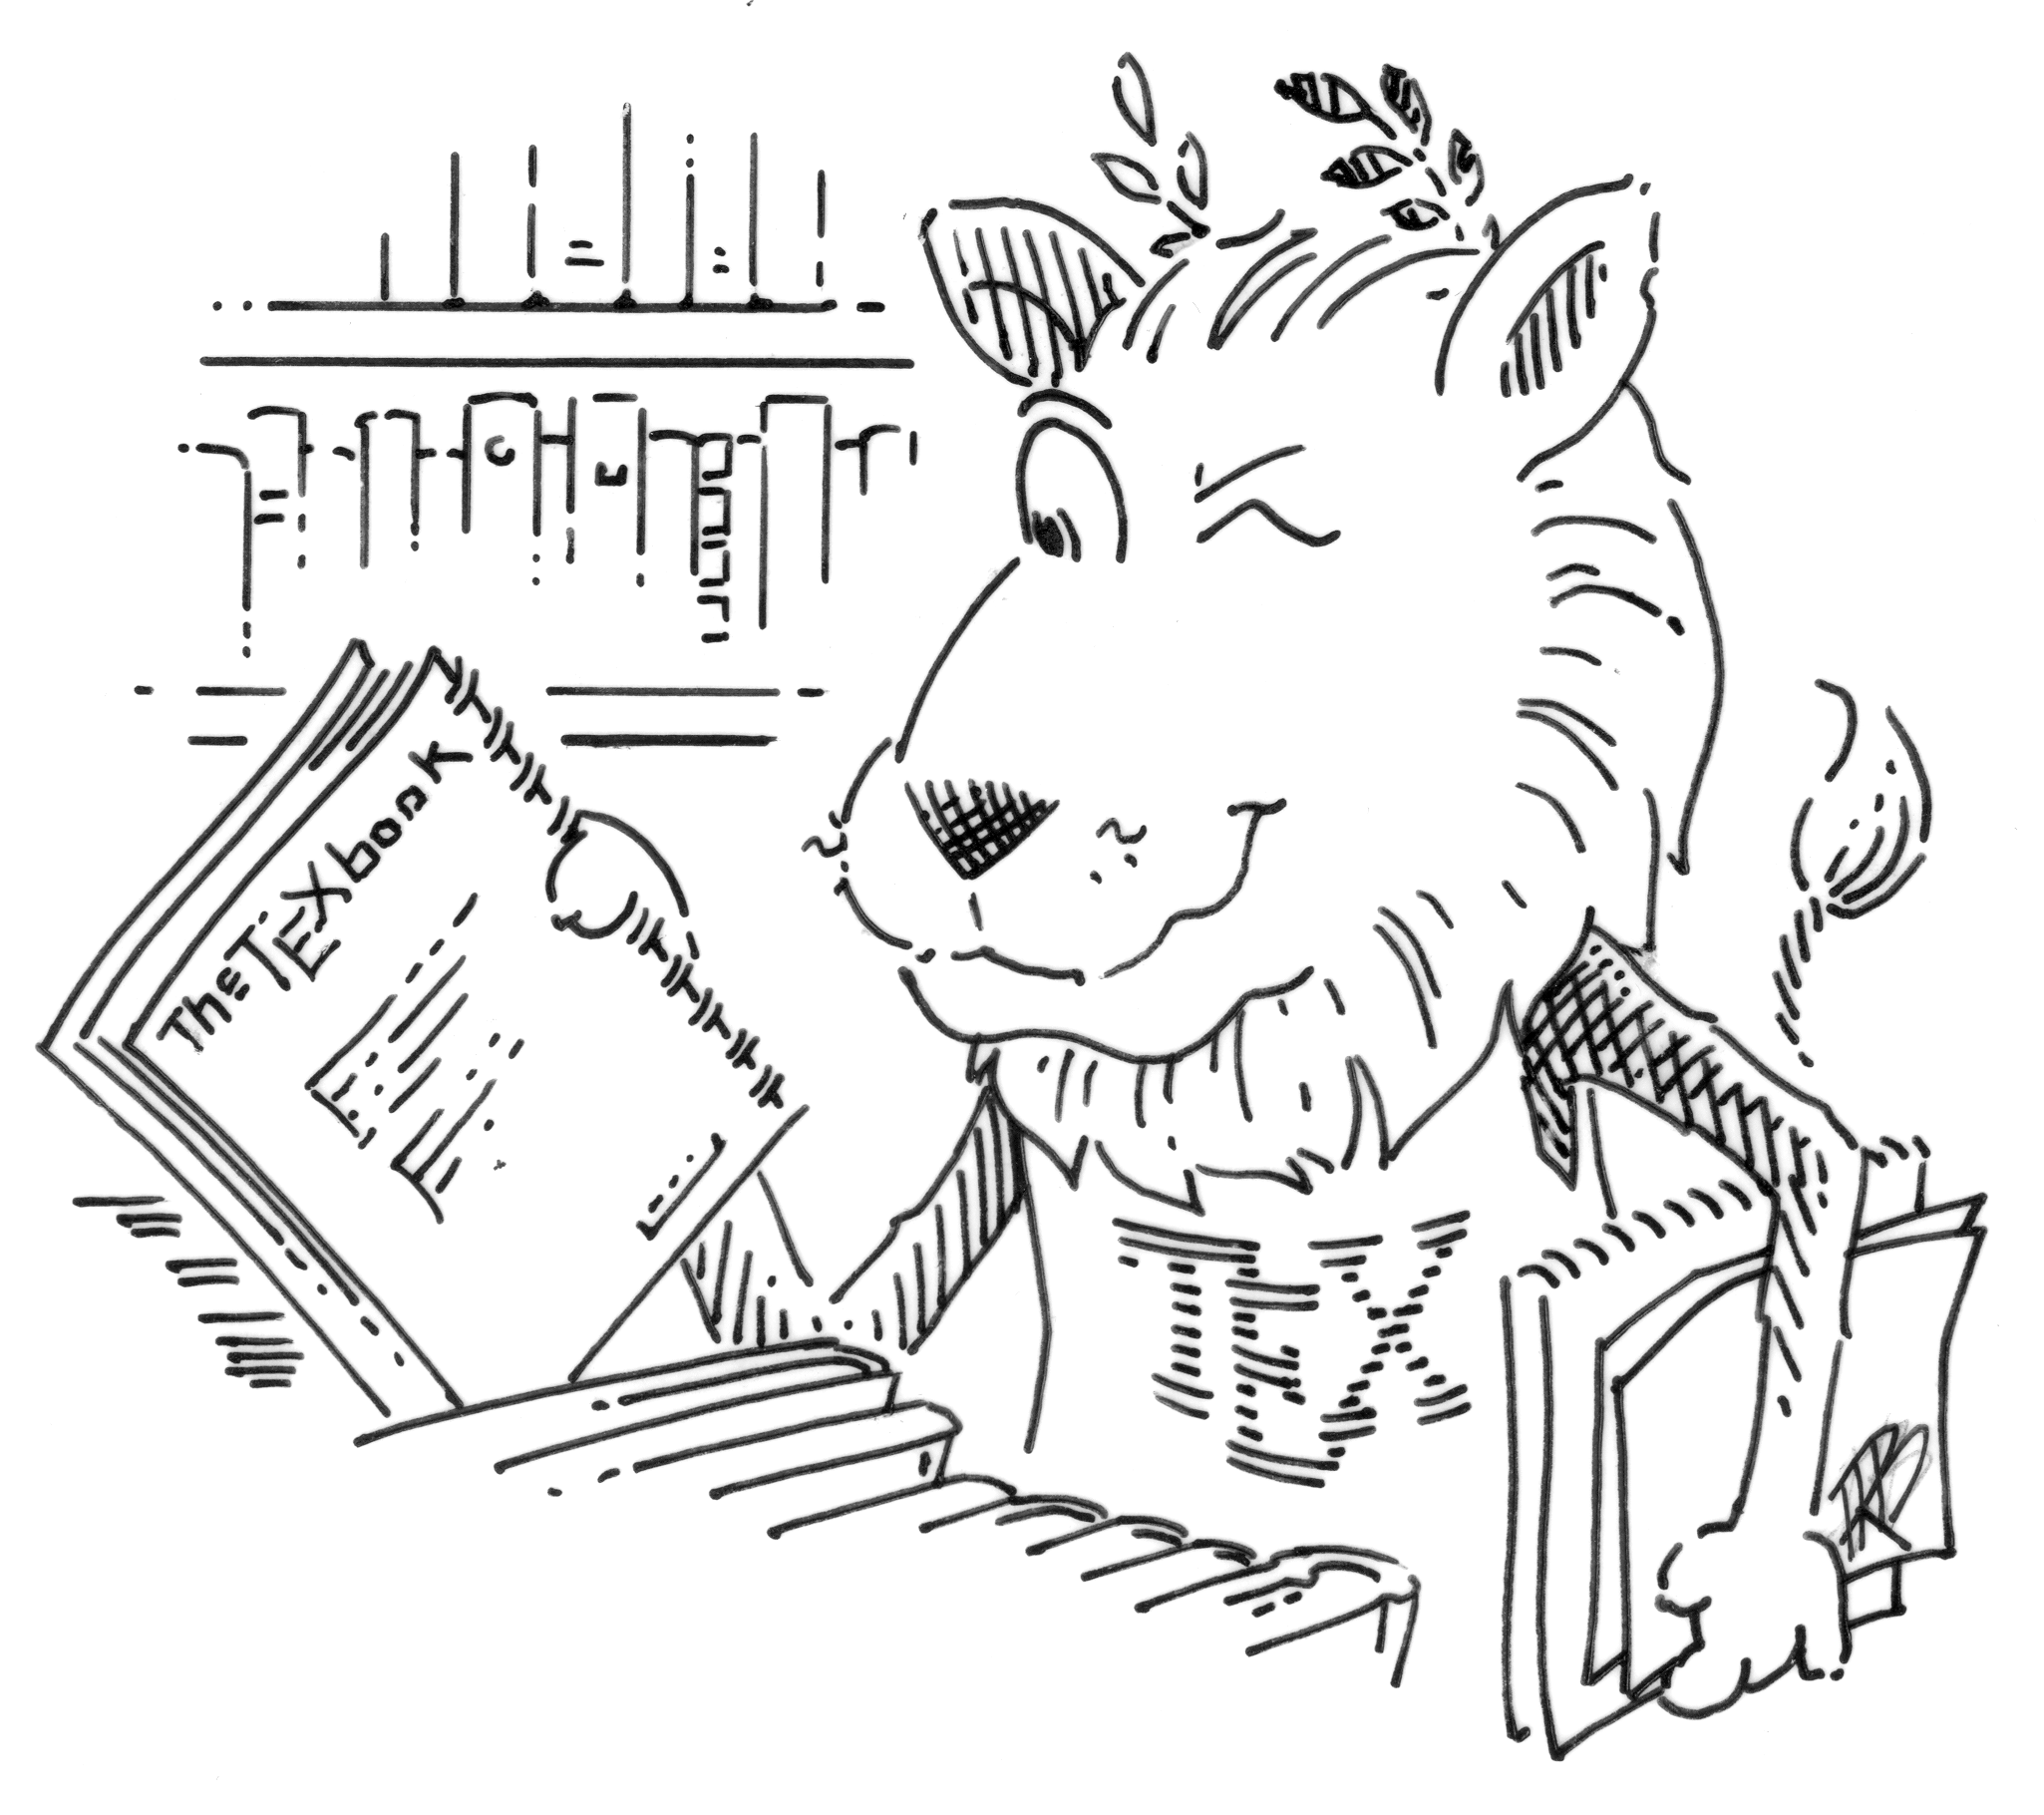
\includegraphics[width=0.8\linewidth]{tex_lion}
		\caption{El león Tex}
		\label{fig:leontex2}
	\end{wrapfigure}
	ggfdg gdfg gd gfdg gfgsgf ggsfg ggsdfg jhgjghjhk kjhgkhgkhg khgkhgkgh kjhkhkggkh khgkhgkh vxcvx cvxcv xcbcbvc bvcbv cbcvvnv nbmbn mnbmn bmn bmnb nbmnbmnb mn mnb mnbmbnmnb.
	ggfdg gdfg gd gfdg gfgsgf ggsfg ggsdfg jhgjghjhk kjhgkhgkhg khgkhgkgh kjhkhkggkh khgkhgkh vxcvx cvxcv xcbcbvc bvcbv cbcvvnv nbmbn mnbmn bmn bmnb nbmnbmnb mn mnb mnbmbnmnb.
	ggfdg gdfg gd gfdg gfgsgf ggsfg ggsdfg jhgjghjhk kjhgkhgkhg khgkhgkgh kjhkhkggkh khgkhgkh vxcvx cvxcv xcbcbvc bvcbv cbcvvnv nbmbn mnbmn bmn bmnb nbmnbmnb mn mnb mnbmbnmnb.
	
	ggfdg gdfg gd gfdg gfgsgf ggsfg ggsdfg jhgjghjhk kjhgkhgkhg khgkhgkgh kjhkhkggkh khgkhgkh vxcvx cvxcv xcbcbvc bvcbv cbcvvnv nbmbn mnbmn bmn bmnb nbmnbmnb mn mnb mnbmbnmnb.
	ggfdg gdfg gd gfdg gfgsgf ggsfg ggsdfg jhgjghjhk kjhgkhgkhg khgkhgkgh kjhkhkggkh khgkhgkh vxcvx cvxcv xcbcbvc bvcbv cbcvvnv nbmbn mnbmn bmn bmnb nbmnbmnb mn mnb mnbmbnmnb.
	
	\end{minipage}
	
	\clearpage
	\section{Texto sobre una figura}
	
	ggfdg gdfg gd gfdg gfgsgf ggsfg ggsdfg jhgjghjhk kjhgkhgkhg khgkhgkgh kjhkhkggkh khgkhgkh vxcvx cvxcv xcbcbvc bvcbv cbcvvnv nbmbn mnbmn bmn bmnb nbmnbmnb mn mnb mnbmbnmnb.
	ggfdg gdfg gd gfdg gfgsgf ggsfg ggsdfg jhgjghjhk kjhgkhgkhg khgkhgkgh kjhkhkggkh khgkhgkh vxcvx cvxcv xcbcbvc bvcbv cbcvvnv nbmbn mnbmn bmn bmnb nbmnbmnb mn mnb mnbmbnmnb.
	
	\begin{figure}[h]
		\color{colorGris1}\centering
		\begin{overpic}[width=0.6\linewidth, tics=5, grid]{plot}
			% Borrar grilla se quita el comando grid 
			\put (20,1) {5}
			\put (40,1) {10}
			\put (60,1) {15}
			\put (80,1) {20}
			\put (0,20) {5}
			\put (0,40) {10}
			\put (0,60) {15}
			\put (63,67) {$ \boxed{f(x) = x^3} $}
		\end{overpic}
		\caption{Gráfico de una función}
		\label{fig:funcion1}
	\end{figure}
	
	ggfdg gdfg gd gfdg gfgsgf ggsfg ggsdfg jhgjghjhk kjhgkhgkhg khgkhgkgh kjhkhkggkh khgkhgkh vxcvx cvxcv xcbcbvc bvcbv cbcvvnv nbmbn mnbmn bmn bmnb nbmnbmnb mn mnb mnbmbnmnb.
	ggfdg gdfg gd gfdg gfgsgf ggsfg ggsdfg jhgjghjhk kjhgkhgkhg khgkhgkgh kjhkhkggkh khgkhgkh vxcvx cvxcv xcbcbvc bvcbv cbcvvnv nbmbn mnbmn bmn bmnb nbmnbmnb mn mnb mnbmbnmnb.
	ggfdg gdfg gd gfdg gfgsgf ggsfg ggsdfg jhgjghjhk kjhgkhgkhg khgkhgkgh kjhkhkggkh khgkhgkh vxcvx cvxcv xcbcbvc bvcbv cbcvvnv nbmbn mnbmn bmn bmnb nbmnbmnb mn mnb mnbmbnmnb.
	ggfdg gdfg gd gfdg gfgsgf ggsfg ggsdfg jhgjghjhk kjhgkhgkhg khgkhgkgh kjhkhkggkh khgkhgkh vxcvx cvxcv xcbcbvc bvcbv cbcvvnv nbmbn mnbmn bmn bmnb nbmnbmnb mn mnb mnbmbnmnb. \footnote{\textcolor{colorAzul1}Justo está bueno poner una nota al pie de página.}
	
	\section{El entorno table}
	
	\begin{table}[h]
		\centering
		\caption{Ejemplo de tabla.}
		\begin{tabular}{|c|c|c|c|}
			\hline
			& 1 & 2 & 3 \\
			\hline
			A & & & \\
			\hline
			B & & & \\
			\hline
		\end{tabular}
		\label{tab:datos}
	\end{table}
	Esta es la referencia a la tabla \ref{tab:datos}
	
	\section{Personalizar tablas}
	
	ggfdg gdfg gd gfdg gfgsgf ggsfg ggsdfg jhgjghjhk kjhgkhgkhg khgkhgkgh kjhkhkggkh khgkhgkh vxcvx cvxcv xcbcbvc bvcbv cbcvvnv nbmbn mnbmn bmn bmnb nbmnbmnb mn mnb mnbmbnmnb.
	
	% Tabla sin personalizar
	\begin{table}[h]
		\centering
		\caption{Coeficientes parciales de seguridad en ELS.}
		\begin{tabular}{p{4cm}cc}
			\hline \textbf{Tipo de acción} & \textbf{Efecto desfavorable} & \textbf{Efecto favorable} \\
			\hline Permanente & gG=1 & gG=1 \\
			\hline Pretensado & 1.10 & 0.90 \\
			\hline Permanente de valor no constante & 1.00 & 1.00 \\
			\hline Variable &.00 & 0.00 \\
			\hline
		\end{tabular}
		\label{tab:coeficientes1}
	\end{table}
	
	Esta es la referencia a la tabla \ref{tab:datos}
	
	% Tabla sin personalizada
	\begin{table}[h]
		\centering
		\caption{Coeficientes parciales de seguridad en ELS.}
		\rowcolors{1}{white}{gray}
		\arrayrulecolor{colorAzul1}
		{\color{colorAzul1}
		\begin{tabular}{p{4cm}cc}
			\toprule % Primera línea
			\hline \textbf{Tipo de acción} & \textbf{Efecto desfavorable} & \textbf{Efecto favorable} \\
			\midrule % Segunda línea
			Permanente & $ \gamma_G= $1.00 & $ \gamma_G= $1.00 \\
			Pretensado & 1.10 & 0.90 \\
			Permanente de valor no constante & 1.00 & 1.00 \\
			Variable &.00 & 0.00 \\
			\bottomrule % Última línea
		\end{tabular}}
		\label{tab:coeficientes2}
	\end{table}
	
	Esta es la referencia a la tabla \ref{tab:datos}
	
	
	sfsdafa sagdgdf ggfdg gdfg gd gfdg gfgsgf ggsfg ggsdfg jhgjghjhk kjhgkhgkhg khgkhgkgh kjhkhkggkh khgkhgkh vxcvx cvxcv xcbcbvc bvcbv cbcvvnv nbmbn mnbmn bmn bmnb nbmnbmnb mn mnb mnbmbnmnb.
	
	\section{Excel2LaTeX}
	
	ggfdg gdfg gd gfdg gfgsgf ggsfg ggsdfg jhgjghjhk kjhgkhgkhg khgkhgkgh kjhkhkggkh khgkhgkh vxcvx cvxcv xcbcbvc bvcbv cbcvvnv nbmbn mnbmn bmn bmnb nbmnbmnb mn mnb mnbmbnmnb.
	
	% Table generated by Excel2LaTeX from sheet 'Sheet1'
	\begin{table}[htbp]
		\centering
		\caption{Tablas de excel}
		\begin{tabular}{p{2.39em}p{15.28em}lllr}
			\multicolumn{1}{l}{} & \multicolumn{1}{r}{} & \multicolumn{4}{c}{\textbf{2021}} \\
			\midrule
			\textbf{Etapa} & \textbf{Productos/Entregables} & \multicolumn{1}{p{4.055em}}{\textbf{Ene-Mar}} & \multicolumn{1}{p{4.055em}}{\textbf{Abr-Jun}} & \multicolumn{1}{p{4.055em}}{\textbf{Jul-Set}} & \multicolumn{1}{p{4.055em}}{\textbf{Oct-Dic}} \\
			\midrule
			E1    & Primer documento a entregar, en .doc. &       & \cellcolor[rgb]{ .718,  .871,  .91} &       &  \\
			E2    & Segundo documento, más pesado. & \cellcolor[rgb]{ .776,  .89,  .859} &       &       &  \\
			E2    & Este tema mejor que no falte. &       & \cellcolor[rgb]{ .776,  .89,  .859} &       &  \\
			E2    & Otro tema interesante en PDF. &       &       & \cellcolor[rgb]{ .776,  .89,  .859} &  \\
			E2    & Esto es importante, también va. &       &       & \cellcolor[rgb]{ .776,  .89,  .859} &  \\
			E3    & Un documento para ver como vamos, editable. &       & \cellcolor[rgb]{ .722,  .804,  .894} &       &  \\
			E4    & Informe de evaluación hasta ahora. &       & \cellcolor[rgb]{ .722,  .804,  .894} &       &  \\
			E5    & Diseño final del sistema. &       &       &       & \cellcolor[rgb]{ .722,  .804,  .894} \\
			E6    & Recomendaciones estratégicas. &       &       &       & \cellcolor[rgb]{ .722,  .804,  .894} \\
			\bottomrule
		\end{tabular}%
		\label{tab:cronograma}%
	\end{table}%
		final de la tabla gdfg gd gfdg gfgsgf ggsfg ggsdfg jhgjghjhk kjhgkhgkhg khgkhgkgh kjhkhkggkh khgkhgkh vxcvx cvxcv xcbcbvc bvcbv cbcvvnv nbmbn mnbmn bmn bmnb nbmnbmnb mn mnb mnbmbnmnb.
	
	\newpage
	\section{Referencias cruzadas}
	Esta es la referencia a la \autoref{tab:cronograma} en la \autopageref{tab:cronograma}.
	
	ggfdg gdfg gd gfdg gfgsgf ggsfg ggsdfg jhgjghjhk kjhgkhgkhg khgkhgkgh kjhkhkggkh khgkhgkh vxcvx cvxcv xcbcbvc bvcbv cbcvvnv nbmbn mnbmn bmn bmnb nbmnbmnb mn mnb mnbmbnmnb.
	
	ggfdg gdfg gd gfdg gfgsgf ggsfg ggsdfg jhgjghjhk kjhgkhgkhg khgkhgkgh kjhkhkggkh khgkhgkh vxcvx cvxcv xcbcbvc bvcbv cbcvvnv nbmbn mnbmn bmn bmnb nbmnbmnb mn mnb mnbmbnmnb.
	
	\section{Mini páginas}
	\begin{center}
		\begin{minipage}{0.47\linewidth} % Para que puedan entrar dos minipaginas en columnas
		\includegraphics[width=1\linewidth]{example-image-a}
	\end{minipage}
	\begin{minipage}{0.47\linewidth}
		\includegraphics[width=1\linewidth]{example-image-b}
	\end{minipage}
	\end{center}
	
	\begin{center}
		\begin{minipage}{0.47\linewidth} % Para que puedan entrar dos minipaginas en columnas
			\includegraphics[width=1\linewidth]{example-image-a}
			\captionof{figure}{Leyenda de la figura A.}
		\end{minipage}\hfil
		\begin{minipage}{0.3\linewidth}
			ggfdg gdfg gd gfdg gfgsgf ggsfg ggsdfg jhgjghjhk kjhgkhgkhg khgkhgkgh kjhkhkggkh khgkhgkh vxcvx cvxcv xcbcbvc bvcbv cbcvvnv nbmbn mnbmn bmn bmnb nbmnbmnb mn mnb mnbmbnmnb
		\end{minipage}
	\end{center}
	
	\section{Entorno matemático}
	ggfdg gdfg gd gfdg gfgsgf ggsfg ggsdfg jhgjghjhk kjhgkhgkhg khgkhgkgh kjhkhkggkh khgkhgkh vxcvx cvxcv xcbcbvc bvcbv cbcvvnv nbmbn mnbmn bmn bmnb nbmnbmnb mn mnb mnbmbnmnb. La ecuación $ E = m \cdot c^2 $.
	
	Tenemos también $ f_{yk} $ o sino $ x_{a}^{2} $, también tenemos $ \frac{2}{4} $ o sino $ \dfrac{3}{4} $ o la raíz $-\sqrt{2}$, centrar la siguiente ecuación el línea aparte y fuera del párrafo: $$E = m \cdot c^2 $$
	
	La ecuación \ref{eq:energía} se referencia solo el número, pero podemos escribir todo así \autoref{eq:energía} o sino la utilizada en los libros que es así: \eqref{eq:energía}
	
	Numerar ecuaciones en su propio entorno:
	\begin{equation} \label{eq:energía}
		E = m \cdot c^2
	\end{equation}
	
	Ecuación sin numerar dentro de un entorno
	\begin{equation*}
		E = m \cdot c^2
	\end{equation*}
	
	
	\section{Símbolos}
	La suma es $ a + b $, la resta es $ a - b $, la multiplicación es $ a \cdot b$ o sino $ a \times b $
	
	Para funciones trigonométricas $ \cos(30) $ o sino $ \sin(30) $
	
	Para integrales $$ \int_0^L x^2, \quad \quad 10 < 15 \quad \Rightarrow \quad 15 \geq 10 $$ % El comando \quad es para dar un espacio en blanco pero se puede utilizar también el comando \hspace{4} donde el 4 es la cantidad de espacios.
	
	\section{Matrices y arreglos}
	
	Ecuaciones alineadas y numeradas
	\begin{align}
		f(x) & = x^2 + x^3 \\
		& = x^2 + x^2 \cdot x
	\end{align}
	
	Ecuaciones alineadas y no numeradas
	\begin{align*}
		f(x) & = x^2 + x^3 \\
		& = x^2 + x^2 \cdot x
	\end{align*}
	
	Matrices numeradas
	\begin{equation}
		A = 
		\begin{pmatrix}
			1 & 2 & 3 \\
			4 & 5 & 6 \\
			7 & 8 & 9
		\end{pmatrix}
	\end{equation}
	
	Matrices no numeradas
	\begin{equation*}
		A = 
		\begin{pmatrix}
			1 & 2 & 3 \\
			4 & 5 & 6 \\
			7 & 8 & 9
		\end{pmatrix}, \quad
		B = 
		\begin{bmatrix}
			1 & 2 & 3 \\
			4 & 5 & 6 \\
			7 & 8 & 9
		\end{bmatrix}, \quad
		C = 
		\begin{matrix}
		1 & 2 & 3 \\
		4 & 5 & 6 \\
		7 & 8 & 9
		\end{matrix}, \quad
		D = 
		\begin{Bmatrix}
		1 & a & 3 \\
		4 & b_2 & 6 \\
		7 & 8 & 9
		\end{Bmatrix}, \quad
		E = 
		\begin{vmatrix}
		1 & 2 & 3 \\
		4 & 5 & 6 \\
		7 & 8 & 9
		\end{vmatrix}, \quad
		F = 
		\begin{Vmatrix}
		1 & 2 & 3 \\
		4 & 5 & 6 \\
		7 & 8 & 9
		\end{Vmatrix}
	\end{equation*} % No tiene que quedar la línea en blanco o sino sale error
	
	\section{Dibujar ecuaciones con la mano}
	Ir a asistentes y después asistente de matemáticas ... que está al final del menú.
	No olvidar poner el entorno equation para escribir en lenguaje matemático.
	\begin{equation}
		\sum _{x=0}^{n}f{\left(x\right)}^{2}+1=0
	\end{equation}
	
	\section{Tipos de errores y alertas}
	
		Undefined control sequence.- No conoce el comando. Está mal escrito o no está cargado el paquete necesario.
	
		Missing \$ inserted.- Falta el entorno matemático.
	
		Extra \} or forggotten \$.- Falta cerrar una viñeta o entorno matemático.
	
		File ended while scannig. . ..- Algo empezó con { pero nunca se cerró.
		
		llegal unit of measure.- No se indicó una unidad de medida o distancia o no existe.
		
		File ‘nombre’ not found.- No se encuentra un archivo. No existe o está mal escrito.
		
		Extra alignment tab has been changed to $\backslash$cr.- Faltan o sobran columnas en una tabla.
		
		Environment ‘nombre’ undefined.- No existe o se escribió mal un entorno.\newline
		
		ADVERTENCIAS
		
		No position in optional float specifier.- No se indició posición en figura o tabla [hbtp!].
		
		Reference ‘nombre’ undefined.- No se encuentra una referencia. No existe o está mal escrita.
		
		There were multiply-defined labels.- Cuando tenemos más de un elemento con la misma etiqueta.
		
		\section{Estructura de carpetas}
		\begin{enumerate}
			\item Bibliografía
			\item Figuras
			\item Secciones
			\item Settings o ajustes
		\end{enumerate}
		
		\section{Unir muchos archivos}
		
		\begin{itemize}
			\item paquetes.tex
			\item inicial.tex
			\item 00\_portada.tex
			\item 01\_introducción.tex
			\item 02\_metodología.tex
			\item 03\_conclusiones.tex
		\end{itemize}
		
		\section{Ventajas del sistema}
		
		\section{Bibliografía a mano}
		\addcontentsline{toc}{section}{Referencias} % Para que salga en el índice
		
		
		ggfdg gdfg gd gfdg gfgsgf ggsfg ggsdfg jhgjghjhk kjhgkhgkhg khgkhgkgh kjhkhkggkh khgkhgkh vxcvx cvxcv xcbcbvc bvcbv cbcvvnv nbmbn mnbmn bmn bmnb nbmnbmnb mn mnb mnbmbnmnb. Como dijo \cite{notsoshort}. Tengo también a \cite{typogra} o a los dos \cite{notsoshort, typogra}.
		
		\begin{thebibliography}{100} % Indica que se van a poner 100 referencias bibliográficas
			\bibitem{notsoshort} \textit{The not So Short Introduction to \LaTeX}, Oetiker, T. et.al., 2015.
			\bibitem{typogra} \textit{Digital Typography Using \LaTeX}, Syropoulos, A., Tsolomitis, et.al., Springer NY, 2003.
		\end{thebibliography}
		
		\section{El paquete BibLaTeX}
		$\backslash$usepackage\{biblatex\}
		
		ggfdg gdfg gd gfdg gfgsgf ggsfg ggsdfg jhgjghjhk kjhgkhgkhg khgkhgkgh kjhkhkggkh khgkhgkh vxcvx cvxcv xcbcbvc bvcbv cbcvvnv nbmbn mnbmn bmn bmnb nbmnbmnb mn mnb mnbmbnmnb. Como dijo \cite{ArgosyMedicalAnimation} y también \parencite{article-example, biber, biblatex} y por otra parte \textcite{guia1}.
		
		% Bibliografía del paquete BibLaTeX
		\printbibliography[heading=bibintoc]
		
		\begin{tikzpicture}
			{\draw (0mm,0mm);}
			{\shade [inner color=red, outer color=white, even odd rule] circle (15mm) circle (2mm);}
			{\fill[red] (15, -3) circle (10mm);}
			%{\draw[->](-1.5,0) -- (1.5,0);}
			%{\draw[->](0,-1.5) -- (0,1.5);}
			{\shadedraw[shading=radial, line width=2mm, color=blue, outer color=red, inner color=yellow](10,-3) circle (30mm);}
		\end{tikzpicture}
\end{document}